\chapter{Second-Order Systems}


So far we've seen first-order differential equations and systems of first-order ODEs.  In this chapter, we'll introduce second-order systems, which are particularly useful for modeling Newtonian motion.

\index{Newtonian motion}
\index{Newton's law of motion}

\section{Newtonian Motion}

Newton's second law of motion is often written like this:

\begin{equation*}
    F = m a
\end{equation*}
where $F$ is the net force acting on an object, $m$ is the
mass of the object, and $a$ is the acceleration of the object.

This equation suggests
that if you know $m$ and $a$, you can compute the force. And that's true,
but in most physical simulations it's the other way around: based on a
physical model, you know $F$ and $m$, and you compute $a$.

\index{second derivative}
\index{second-order differential equation}
\index{differential equation!second-order}

So if we know acceleration as a function of time, how do we
find the position of the object, $r$?  Well, we know that acceleration
is the second derivative of position, so we can write the differential
equation

\begin{equation*}
    \frac{d^2r}{dt^2} = a
\end{equation*}
where ${d^2r}/{dt^2}$ is the second time derivative of $r$.

Because this equation includes a second derivative, it's
a second-order ODE.  We can't solve the equation using \lstinline{ode45} in this form, but
by introducing a new variable, \emph{v}, for velocity, we can rewrite it
as a system of first-order ODEs:

\begin{eqnarray*}
    \frac{dr}{dt} &=& v   \\
    \frac{dv}{dt} &=& a
\end{eqnarray*}

The first equation says that the first derivative of $r$ is $v$;
the second equation says that the first derivative of $v$ is $a$.


\section{Free Fall}
\label{freefall}

As an example of Newtonian motion, let's go back to the question from Section~\ref{penny}:

\begin{quote}
If you drop a penny from the top of the Empire State Building, how long does it take to reach the sidewalk, and how fast is it going when it gets there?
\end{quote}

We'll start with no air resistance; then we'll add air resistance to the model and see what effect it has.

\index{air resistance}
\index{gravity}

Near the surface of the earth,
acceleration due to gravity is \SI{-9.8}{\meter \per \second \squared}, where the minus sign
indicates that gravity pulls down.
If the object falls straight down, we can describe its position with a
scalar value $y$, representing altitude.

\index{position}
\index{velocity}
\index{rate function}
Listing~\ref{lst:penny_rate_func} contains a rate function we can use with \lstinline{ode45} to solve
this problem:

\begin{lstlisting}[caption={A rate function for the falling penny problem}, label={lst:penny_rate_func}]
function res = rate_func(t, X)
    % unpack position and velocity
    y = X(1);
    v = X(2);

    % compute the derivatives
    dydt = v;
    dvdt = -9.8;

    % pack the derivatives into a column vector
    res = [dydt; dvdt];
end
\end{lstlisting}

The rate function in Listing~\ref{lst:penny_rate_func} takes \lstinline{t} and \lstinline{X} as input variables, where the elements of \lstinline{X} are understood to be the position and velocity of the penny.

It returns a column vector that contains \lstinline{dydt} and \lstinline{dvdt}, which
are velocity and acceleration, respectively.
Since velocity is the second element of \lstinline{X}, we can simply assign this value to \lstinline{dydt}.
And since the derivative of velocity is acceleration, we can assign the acceleration due to gravity to \lstinline{dvdt}.

\index{column vector}
\index{acceleration}

As always, we should test the rate function before we call \lstinline{ode45}.  Here's the top-level function we can use to test it:

\begin{code}
function penny()
   t = 0;
   X = [381, 0];
   rate_func(t, X)
end
\end{code}

The initial condition of \lstinline{X} is the initial position, which is the height of the Empire State Building, about \SI{381}{\meter}, and the initial velocity, which is \SI{0}{\meter \per \second}.

\index{Empire State Building}
\index{penny}

The result from \lstinline{rate_func} is

\begin{code}
    0
   -9.8000
\end{code}
which is what we expect.

Now we can run \lstinline{ode45} with this rate function:

\begin{code}
tspan = [0, 10]
[T, M] = ode45(@rate_func, tspan, X)
\end{code}

As always, the first argument is the function handle, the second
is the time span (10 seconds), and the third is the initial
condition.

The result is a vector, \lstinline{T}, that contains the time values, and a matrix, \lstinline{M}, that contains two columns, one for altitude and one for velocity.
\index{function handle}
\index{time span}
\index{matrix}

We can extract the first column and plot it, like this:

\begin{code}
Y = M(:, 1)
plot(T, Y)
\end{code}


\begin{figure}
\centerline{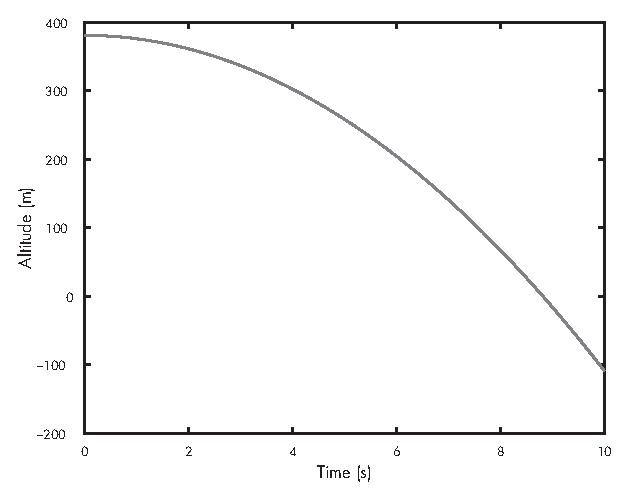
\includegraphics[scale=0.8]{images/figure11_01_new.eps}}
\caption{Altitude versus time for an object in free fall}
\label{fig:penny}
\end{figure}

Figure~\ref{fig:penny} shows the result.  Altitude drops slowly at first and picks up speed.  Between 8 and 9 seconds, the altitude reaches 0, which means the penny hits the sidewalk.  But \lstinline{ode45} doesn't know where the ground is, so  the penny keeps going through 0 into negative altitude.  We'll solve that problem in the next section.

\section{ODE Events}
\label{events}

\index{ODE event}

Normally when you call \lstinline{ode45} you specify a start time and
an end time.  But sometimes you don't know ahead of time when the
simulation should end.  To solve this problem we can define an \emph{event},
something of interest that happens during a simulation,
like the penny reaching the ground.

Here are the steps:

\index{event function}
\index{function!event}
\index{ODE event}

\begin{enumerate}

\item First we define an \emph{event function} that allows \lstinline{ode45} to figure out when
an event occurs.  Here's an event function for the penny example:

\begin{code}
function [value, isterminal, direction] = event_func(t,X)
    value = X(1);
    isterminal = 1;
    direction = -1;
end
\end{code}

The event function takes the same input variables as the rate function and returns three output variables: \lstinline{value} determines when an event can occur, \lstinline{direction} determines whether it does, and \lstinline{isterminal} determines what happens.
More specifically, an event can occur when \lstinline{value} passes through 0.
If \lstinline{direction} is positive, the event only occurs if \lstinline{value} is increasing.
 If \lstinline{direction} is negative, the event only occurs if \lstinline{value} is decreasing.
If \lstinline{direction} is 0, the event always occurs.
If \lstinline{isterminal} is 1, the event causes the simulation to end; if it is 0, the simulation continues.

This event function uses the altitude of the penny as \lstinline{value} so an event can occur when altitude passes through 0.
Because \lstinline{direction} is negative, an event occurs only when altitude is decreasing, and
because \lstinline{isterminal} is 1, the simulation ends if an event occurs.

\index{odeset@\lstinline{odeset}}
\index{options@\lstinline{options}}

\item Next, we use \lstinline{odeset} to create an object called \lstinline{options}:

\begin{code}
options = odeset('Events', @event_func);
\end{code}
%
The name of the option is \lstinline{Events} and the value is the handle of the event function.

\item Finally, we pass \lstinline{options} as a fourth argument to \lstinline{ode45}:

\begin{code}
[T, M] = ode45(@rate_func, tspan, X, options);
\end{code}

When \lstinline{ode45} runs, it invokes \lstinline{event_func} after each time step.  If the event function indicates that a terminal event occurred,
\lstinline{ode45} stops the simulation.

\end{enumerate}

Let's look at the results from the penny example:

\begin{code}
>> T(end)
8.8179

>> M(end, :)
0.0000  -86.4153
\end{code}

The last value of \lstinline{T} is about 8.8, which is the number of seconds the penny takes to reach the sidewalk.

The last row of \lstinline{M} indicates that the final altitude is 0, which is what we wanted, and the final velocity is about \SI{-86}{\meter \per \second}.


\section{Air Resistance}
\label{air_resistance}

\index{drag}
\index{air resistance}

To make this simulation more realistic, we can add air resistance.
For large objects moving quickly through air, the force due to air resistance, called \emph{drag}, is proportional to velocity squared.
For an object falling down, drag is
directed up, so if velocity is negative, drag force is positive.

% b is used in the book "Physics for Scientists and Engineers" by Paul A. Tipler.
%TODO: consider writing out the drag equation

Here's how we can compute the force of drag as a function of velocity in one dimension:

\begin{equation*}
    f_\mathrm{d} = -\mathrm{sign}(v) b v^2
\end{equation*}
where $v$ is velocity and
$b$ is a drag constant that depends on the density of
air, the cross-sectional area of the object, and the shape
of the object.

The sign or signum function returns the value $1$ for positive values of
$v$ and $-1$ for negative values.  So $f_\mathrm{d}$ is always in the opposite direction of $v$.

\index{signum function}
\index{sign@\lstinline{sign}}
\index{mass}
\index{terminal velocity}

To convert from force to acceleration we have to know mass, but that's easy to find: the mass of a penny is about \SI{2.5}{\gram}.  It's not as easy to find the drag constant, but based on reports that the terminal velocity of a penny is about \SI{18}{\meter \per \second}, I've estimated that it's about \SI{75e-6}{\kilogram \per \meter}.

Listing~\ref{lst:acceleration_drag} defines a function that takes \lstinline{t} and \lstinline{X} as input variables and returns the total acceleration of the penny due to gravity and drag:

\begin{lstlisting}[caption={Calculating acceleration of a penny with drag}, label={lst:acceleration_drag}]
function res = acceleration(t, X)
    b = 75e-6;                 % drag constant in kg/m
    v = X(2);                  % velocity in m/s
    f_d = -sign(v) * b * v^2;  % drag force in N

    m = 2.5e-3;               % mass in kg
    a_d = f_d / m;            % drag acceleration in m/s^2

    a_g = -9.8;               % acceleration of gravity in m/s^2
    res = a_g + a_d;          % total acceleration
end
\end{lstlisting}

First, we compute force due to drag .
Then we compute acceleration due to drag .
Lastly, we compute total acceleration due to drag and \mbox{gravity}.

\index{acceleration}
\index{force}

Be careful when you're working with forces and accelerations; make sure
you only add forces to forces or accelerations to accelerations.  In my
code, I use comments to remind myself what units the values have.
That helps me avoid errors like adding forces to accelerations.

To use this function, we make a small change in \lstinline{rate_func}:

\begin{code}
function res = rate_func(t, X)
    y = X(1);
    v = X(2);

    dydt = v;
    dvdt = acceleration(t, X);   % this line has changed

    res = [dydt; dvdt];
end

\end{code}

In the previous version, \lstinline{dvdt} is always \lstinline{-9.8}, the acceleration due to gravity.
In this version, we call \lstinline{acceleration} to compute the total acceleration due to gravity and drag .

\begin{figure}[ht]
\centerline{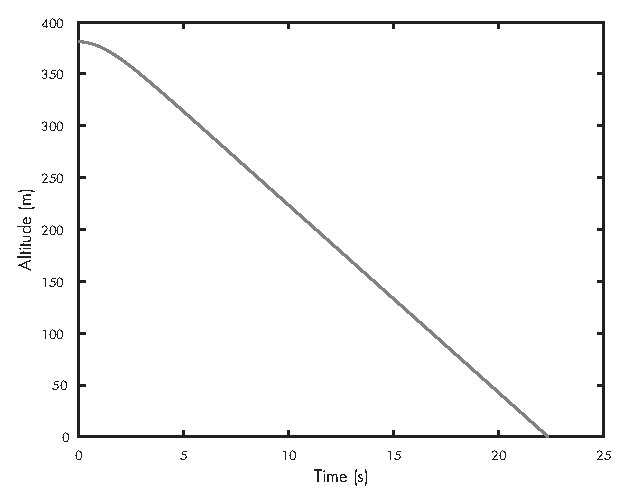
\includegraphics[scale=0.8]{images/figure11_02_new.eps}}
\caption{Altitude versus time for a penny in free fall with air resistance}
\label{fig:penny2}
\end{figure}

Everything else is the same.  Figure~\ref{fig:penny2} shows the result.

Air resistance makes a big difference! Velocity increases until
acceleration due to drag equals acceleration due to gravity; after that, velocity is constant and position decreases linearly (and much more slowly than it would in a vacuum).

With air resistance, the time until the penny hits the sidewalk is \SI{22.4}{\second}, substantially longer than before (\SI{8.8}{\second}).

And the final velocity is \SI{18.1}{\meter \per \second}, substantially slower than before (\SI{86}{\meter \per \second}).

\section{Chapter Review}

In this chapter, we used Newton's laws of motion to write a differential equation that describes the motion of a falling penny.

We rewrote that equation as a system of first-order differential equations so we could use \lstinline{ode45} to solve it.  Then we ran simulations of a falling penny with and without air resistance, also known as \emph{drag}.

We defined an \emph{event} as something of interest that happens during a simulation, like a collision between moving objects, and we wrote an \emph{event function}, which allows \lstinline{ode45} to figure out when an event occurs.

In the next chapter, we extend Newtonian motion to two dimensions and model the flight of a baseball.


\section{Exercises}

Before you go on, you might want to work on the following exercise.

\begin{ex}
\index{skydiver}
\index{parachute}

In this exercise we'll model the descent of a skydiver, taking into account the change in drag when the parachute opens.

\begin{enumerate}

\item Modify the penny code from this chapter to simulate the descent of a \SI{75}{\kilogram} skydiver from an initial altitude of \SI{4000}{\meter}.
The drag constant for a skydiver without a parachute is about \SI{0.2}{\kilogram \per \meter}.
What would the velocity of the skydiver be on impact?

\item After opening their parachute, the velocity of the skydiver slows to about \SI{5}{\meter\per\second}.  Use your simulation to find the drag constant that yields a terminal velocity of \SI{5}{\meter\per\second}.

\item Increase the mass of the skydiver, and confirm that terminal velocity increases.  This phenomenon is the source of the intuition that heavy objects fall faster; in air, they do!

\item Now suppose the skydiver free falls until they get to an altitude of \SI{1000}{\meter} before opening the parachute.  How long would it take them to reach the ground?

\item What is the lowest altitude where the skydiver can open the parachute and still land at less than \SI{6}{\meter\per\second} (assuming that the parachute opens and deploys instantly)?

\end{enumerate}

% skydiver.m

\end{ex}



\begin{ex}
\label{earth}

\index{Earth}
\index{Sun}
\index{Law of Universal Gravitation}

Here's a question from the website \emph{Ask an Astronomer} (see \url{https://greenteapress.com/matlab/astro}):

\begin{quote}
If the Earth suddenly stopped orbiting the Sun, I know eventually it would be pulled in by the Sun's gravity and hit it. How long would it take the Earth to hit the Sun? I imagine it would go slowly at first and then pick up speed.
\end{quote}

Use \lstinline{ode45} to answer this question.  Here are some suggestions about how to proceed:

\begin{enumerate}

\item Look up the Law of Universal Gravitation and any constants you need. I suggest you work entirely in SI units: meters, kilograms, and newtons.

\item When the distance between the Earth and the Sun gets small, this system behaves badly, so you should use an event function to stop when the surface of the Earth reaches the surface of the Sun.

\item Express your answer in days, and plot the results as millions of kilometers versus days.

\end{enumerate}

% earth.m

\end{ex}
